\section{Parameter Estimation With Supernovae}

\begin{enumerate}[label=\textbf{\Alph*}.]
    \item Telescope measures luminosity at different redshifts.
    $\sigma_z \approx 0$.
    Using the data file, determine the best-fit and ``1 sigma'' uncertainty for $\Omega_\Lambda$ from this data.

    Given these equations from the question,
    \begin{align*}
        D &= \frac{1}{H_0} \left(z + \frac{1}{2}z^2 (1-q_0)\right)\\
        q_0 &= \frac{\Omega_M}{2} - \Omega_\Lambda\\
        \Omega_M + \Omega_\Lambda &= 1: \Omega_M, \Omega_\Lambda > 0\\
        L &= \frac{L_0}{D^2}\\
        m &= -2.5\log_{10}(L)\\
        \sigma_m &= \pm 0.1 \\
    \end{align*}

    write $m$ as a function of the other variables:
    \begin{align*}
        m &= -2.5\log_{10}(L)\\
        &= -2.5\log_{10}\left(\frac{L_0}{D^2}\right)\\
        &= -2.5\log_{10}\left(\frac{L_0}{\frac{1}{H_0^2} \left(z + \frac{1}{2}z^2 (1-q_0)\right)^2}\right)\\
        &= -2.5\log_{10}\left(\frac{L_0H_0^2}{\left(z + \frac{1}{2}z^2 \left(1-\left(\frac{\Omega_M}{2} - \Omega_\Lambda\right)\right)\right)^2}\right)\\
        &= -2.5\log_{10}\left(\frac{L_0H_0^2}{\left(z + \frac{1}{2}z^2 \left(\frac{1 + 3\Omega_\Lambda}{2}\right)\right)^2}\right)\\
    \end{align*}

    Since we're given the uncertainty on $m$, let's model this as a Gaussian -- for the mean use the equation above, and we have $\sigma_m$:

    \begin{align*}
        P(m) &= \frac{1}{\sqrt{2\pi}\sigma_m} \exp\left(\frac{-\left(m + 2.5\log_{10}\left(\frac{L_0H_0^2}{\left(z + \frac{1}{2}z^2 (\frac{1 +3 \Omega_\Lambda}{2})\right)^2}\right)\right)^2}{2\sigma_m}\right)
    \end{align*}
    
    \begin{align*}
        &L(\Omega_\Lambda, L_0H_0^2) \\
        &= \prod_i \frac{1}{\sqrt{2\pi}\sigma_m} \exp\left(-\frac{\left(m_i + 2.5\log_{10}\left(\frac{L_0H_0^2}{\left(z_i + \frac{1}{2}z_i^2 (\frac{1 +3 \Omega_\Lambda}{2})\right)^2}\right)\right)^2}{2\sigma_m}\right) \\
        &-\ln L(\Omega_\Lambda, L_0H_0^2) \\
        &= \sum_i \ln(\sqrt{2\pi}\sigma_m) + \left(\frac{\left(m_i + 2.5\log_{10}\left(\frac{L_0H_0^2}{\left(z_i + \frac{1}{2}z_i^2 (\frac{1 +3 \Omega_\Lambda}{2})\right)^2}\right)\right)^2}{2\sigma_m}\right) \\
    \end{align*}

    We can minimize this, to find the best-fit $H_0L_0^2$ and $\Omega_\Lambda$.

    The best-fit values: $\Omega_\Lambda = 0.714, H_0L_0^2 = \SI{4.87e-16}{}$. A plot to make sure the fit actually worked:

    \begin{center}
        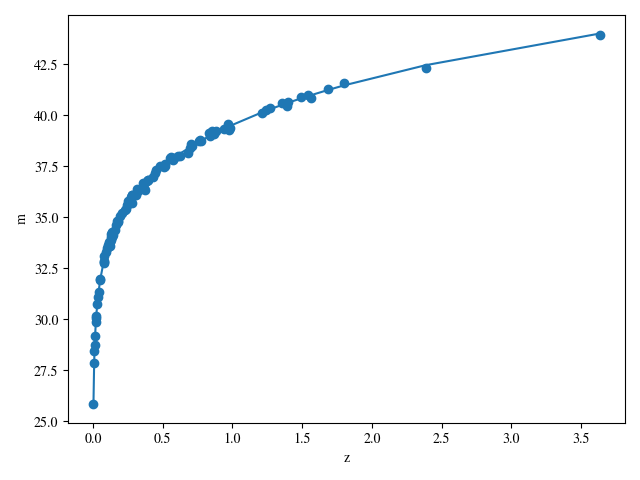
\includegraphics[width=0.75\textwidth]{q3_a_fit.png}
    \end{center}

    We can sub in our best-fit $H_0L_0^2$ and find the points where $-\Delta \ln L = 0.5$ for ``$1\sigma$'' uncertainties.

    See the code for details, but we end up with almost symmetric errors, $+0.0164$ and $-0.0161$:

    $$\Omega_\Lambda = 0.714^{+0.0164}_{-0.0161}.$$

    \begin{center}
        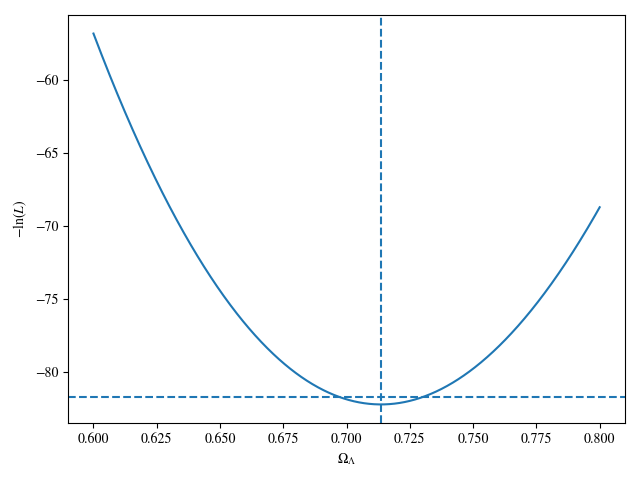
\includegraphics[width=0.75\textwidth]{q3_a_uncert.png}
    \end{center}

    \item Let $L_0(z) = L_0(1+az), a=0 \pm 0.2$. Calculate the new $\Omega_\Lambda$.

    Proceeding in essentially the same way, except making the substitution $L_0 \to L_0(1+az)$ in the likelihood function, and adding an extra term into the likelihood function to deal with the prior on $a$ -- we took a Gaussian prior with mean 0, $\sigma_a=0.2$.

    \begin{align*}
        &-\ln L(\Omega_\Lambda, L_0H_0^2, a) \\
        &= \sum_i \ln(\sqrt{2\pi}\sigma_m) + \left(\frac{\left(m_i + 2.5\log_{10}\left(\frac{L_0(1+az_i)H_0^2}{\left(z_i + \frac{1}{2}z_i^2 (\frac{1 +3 \Omega_\Lambda}{2})\right)^2}\right)\right)^2}{2\sigma_m}\right) \\
        &+ \ln\left(\frac{1}{\sqrt{2\pi}\sigma_a} \exp\left( - \frac{(a - 0)^2}{2\sigma_a^2}\right)\right)
    \end{align*}

    See code for details, we find a ML value of $a=0.0247$ and final result of

    $$\Omega_\Lambda = 0.753^{+0.0166}_{-0.0164}.$$


\end{enumerate}
